%
% CURVAS ELÍPTICAS
%
\section{Curvas Elípticas}

%
% DEFINIÇÃO
%
\subsection{Definição}
Curvas elípticas têm esse nome porque são descritas por equações cúbicas, semelhantes às usadas para calcular a circunferência de uma elipse \cite{Stallings:2011}. Uma curva elíptica \(E\) é um conjunto de soluções de uma equação cúbica definida sobre um corpo \(\mathbb{F}\) é descrita da seguinte forma:
\begin{equation}
y^2 + axy + by = x^3 + cx^2 + dx + e \label{eq:5}
\end{equation}
em que \(a, b, c, d\) e \(e\) são elementos do corpo \(\mathbb{F}\) e \(x\) e \(y\) são as variáveis da equação e assumem valores dentro de \(\mathbb{F}\). A notação utilizada para indicar que uma curva elíptica \(E\) está definida sobre um corpo \(\mathbb{F}\) é $E(\mathbb{F})$, e o corpo \(\mathbb{F}\) é chamado de corpo subjacente da curva \cite{Guide}. Equações deste tipo são conhecidas como \textit{equações de Weierstrass}. Com frequência, no estudo de criptografia de curvas elípticas, costuma-se utilizar a forma reduzida de Weierstrass, descrita pela equação
\begin{equation}
y^2 = x^3 + ax + b \label{eq:6}
\end{equation}
obtida através da mudança de variáveis
\begin{equation}
  (x, y) \rightarrow \left(\frac{x - 3a^2 - 12c}{36},\ \frac{y - 3ax}{216} + \frac{a^3 + 4ac - b}{24}\right)
\end{equation}
e \(\mathbb{F}\) com característica diferente de \(2\) e de \(3\) \cite{Guide}.

É imprescindível que os valores de \(a\) e \(b\) sejam escolhidos tais que $4a^3 + 27b^2 \ne 0$ \cite{Mandy:2007}. Essa condição garante que não existe ponto na curva que possua mais de uma reta tangente, ou seja, a curva é suave(Fig. (~\ref{fig:cuspide})), não possui auto-interseções(curva singular) e nem cúspides \cite{Guide}.
\begin{figure}
%\centering
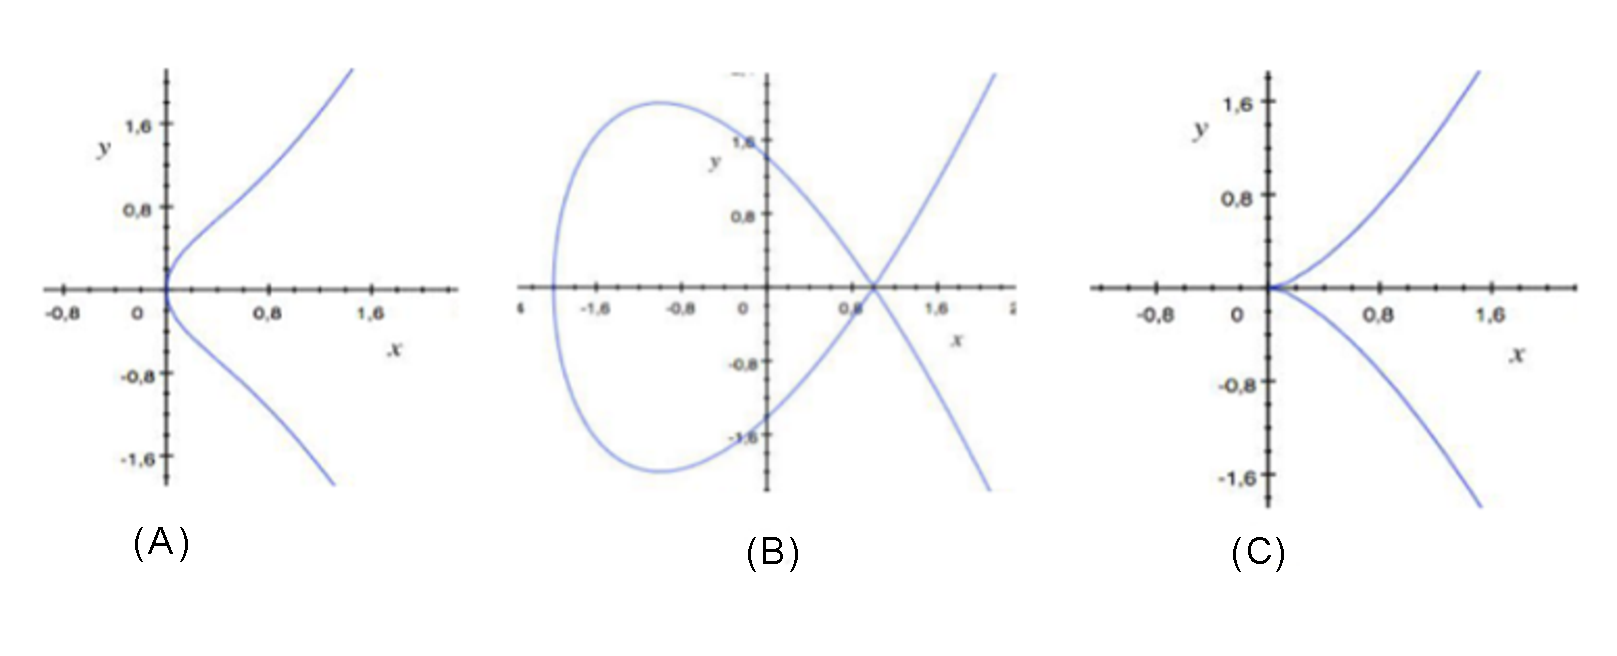
\includegraphics[scale=0.6, bb=0 0 515 478]{figuras/curva_suave_singular_cuspide.eps}
\caption{(A) Curva suave, (B) Curva singular e (C) Cúspide}
\label{fig:cuspide}
\end{figure}

O \textbf{conjunto dos pontos} que pertencem à curva elíptica \(E\) definida sobre um corpo \(\mathbb{F}\) é descrito por:

\begin{equation}
E(\mathbb{F}) = \{(x,y) \in \mathbb{F} \times \mathbb{F} \mid y^2 = x^3 + ax + b\} \cup \{\mathcal{O}\}
\label{eq:pontosCurva}
\end{equation}

em que o ponto $\mathcal{O}$ é chamado de \textit{ponto no infinito}. \cite{Mandy:2007}. Será visto na próxima seção que, juntamente com uma operação de soma dos pontos da curva elíptica, o conjunto $E(\mathbb{F})$ forma um grupo abeliano com o ponto no infinito sendo $\mathcal{O}$ o elemento identidade \cite{Guide}.

A Figura (\ref{fig:curvas}) apresenta alguns exemplos de curvas elípticas usando a forma normal da equação de Weierstrass.

\begin{figure}[h]
\centering
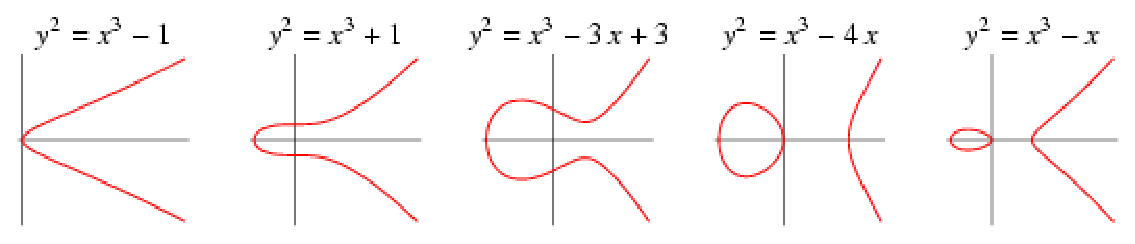
\includegraphics[scale=0.5, bb=0 0 529 101]{figuras/curvas.eps}
\caption{Exemplos de curvas elípticas}
\label{fig:curvas}
\end{figure}

%
% LEIS DE GRUPO PARA CURVAS ELÍPTICAS
%
\subsection{Leis de grupo para Curvas Elípticas}
Seja o conjunto de pontos $E(\mathbb{F})$ da curva elíptica \(E\) definida sobre um corpo \(\mathbb{F}\), é possível definir uma operação sobre esse conjunto de pontos, que será chamada de adição e indicada por $+$. Essa operação de adição e o conjunto de pontos $E(\mathbb{F})$ da curva elíptica formam um grupo abeliano \cite{Stallings:2011}.

A forma mais clara de entender a operação de adição sobre curvas elípticas é geometricamente (ver Fig. (\ref{fig:pontos})). Para somar dois pontos \(P\) e \(Q\) com coordenadas \(x\) diferentes, basta ligar uma linha reta entre eles e encontrar o terceiro ponto de interseção \(R\). Pela natureza das curvas elípticas, pode-se observar que existe um único ponto \(R\) que é o ponto de interseção (a menos que os pontos \(P, Q\) possuam a mesma coordenada $x$ e coordenadas $y$ diferentes). Para formar uma estrutura de grupo, é preciso  definir a adição sobre três pontos da seguinte forma: $P+Q=-R$. \cite{Stallings:2011}

Se as coordenadas \(x\) dos pontos \(P\) e \(Q\) são iguais e as coordenadas $y$ são diferentes, então a reta que passa pelos dois pontos não intersecta a curva elíptica em nenhum outro ponto. Para definir a estrutura de grupo, considera-se que essa reta vertical intersecta a curva no ponto no infinito $\mathcal{O}$. \cite{Stallings:2011}

É possível calcular o dobro de um ponto \(P\), ou seja, calcular a soma do ponto com ele mesmo. Para isso desenha-se a reta tangente à curva no ponto \(P\). Essa linha intersecta a curva elíptica num segundo ponto, que será refletido para obter-se o ponto \(R\), que é o resultado da soma. \cite{Guide} Observe que esse caso se aplica quando se deseja somar os pontos $P$ e $Q$ em que $P=Q$.

\begin{figure}[h]
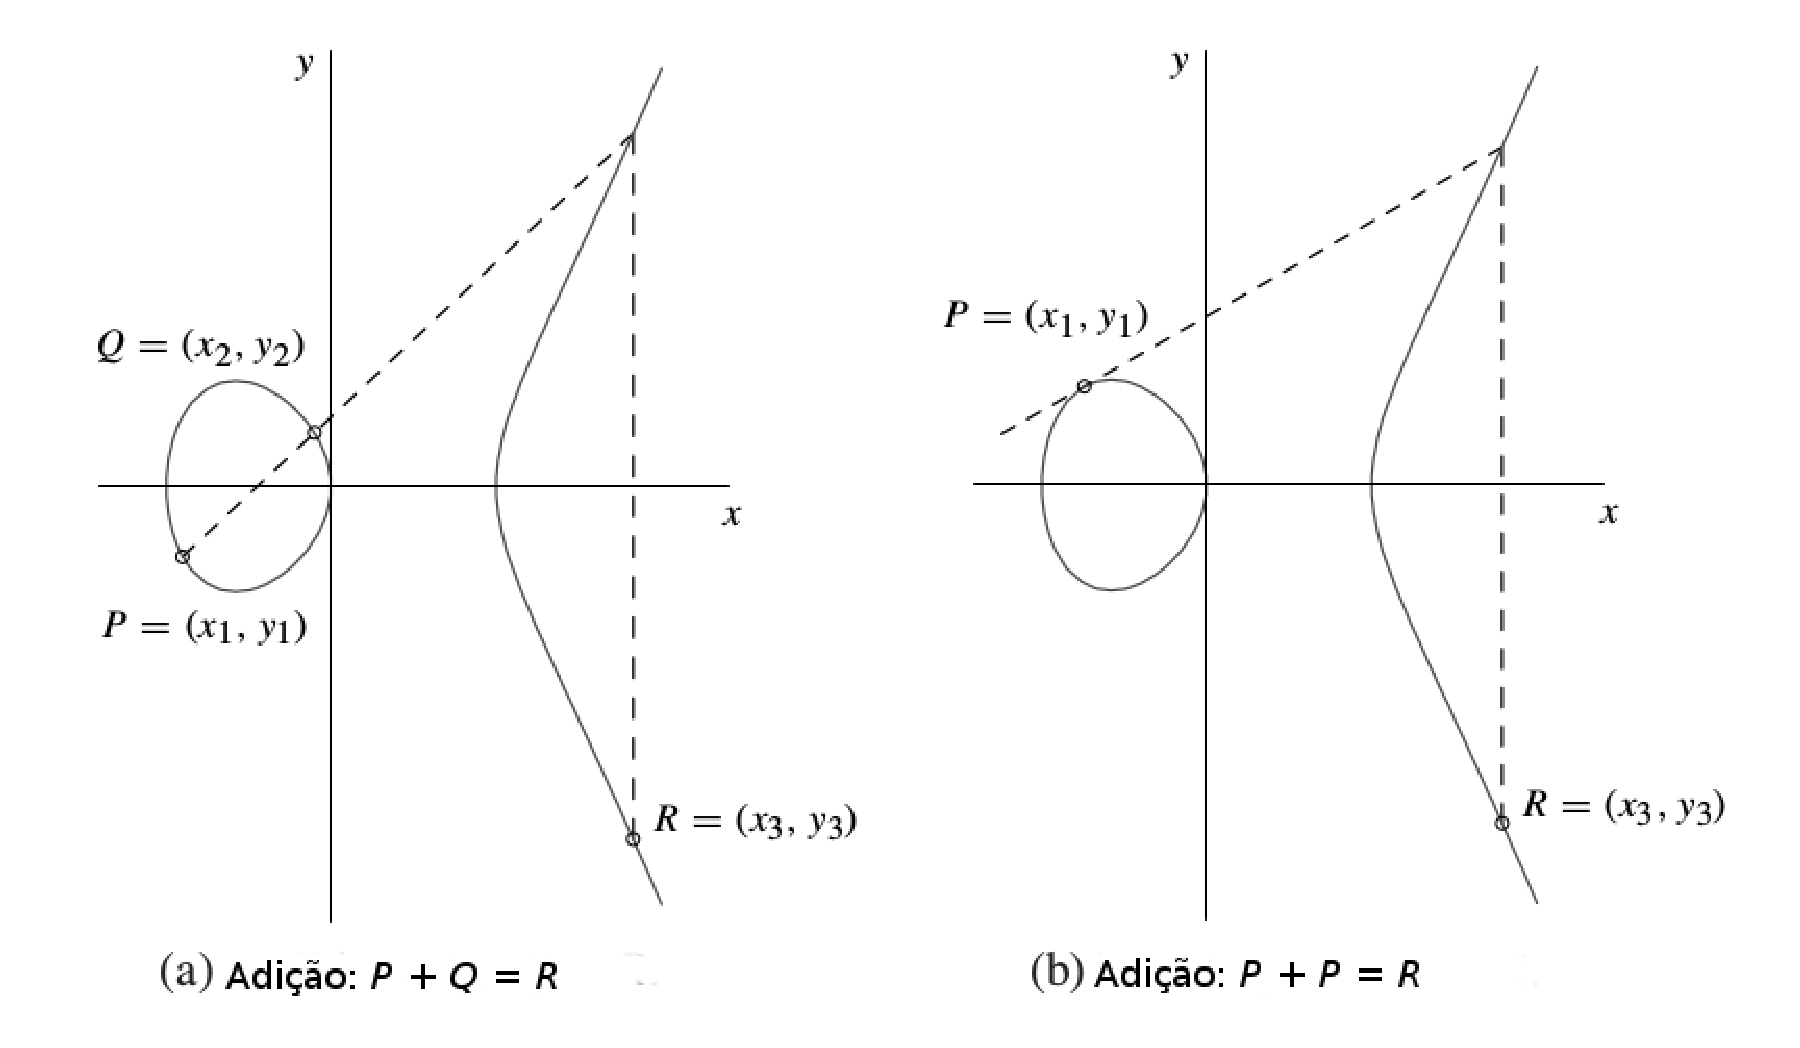
\includegraphics[scale=0.5, bb=0 0 484 636]{figuras/SomaECC.eps}
\caption{Soma de pontos em curvas elípticas}
\label{fig:pontos}
\end{figure}

Os axiomas de grupo são satisfeitos da seguinte forma:
\begin{enumerate}
  \item Para quaisquer pontos $P, Q \in E(\mathbb{F})$, o ponto $P + Q \in E(\mathbb{F})$.
  \item $\mathcal{O}$ é o elemento identidade. Logo, $P + \mathcal{O} = P$ para todo $P \in E(\mathbb{F})$.
  \item Para qualquer ponto \(P\), existe um ponto $P'$ tal que $P + P' = \mathcal{O}$. O ponto $P'$ é denominado \textit{inverso aditivo} de \(P\).
  \item A adição é associativa. Logo, $P, Q, R \in E(\mathbb{F})$, observa-se que $(P + Q) + R = P + (Q + R)$
  \item A adição é comutativa. Logo, $P, Q \in E(\mathbb{F})$, observa-se que $P + Q = Q + P$.
\end{enumerate}

%
% CURVAS ELÍPTICAS SOBRE CORPO FINITO
%
\subsection{Curvas elípticas sobre corpo finito}
A criptografia de curva elíptica utiliza curvas elípticas em que as variáveis e coeficientes são restritos a elementos de um corpo finito \cite{Stallings:2011}, ou seja, sendo a curva elíptica $E$ definida sobre o corpo finito $\mathbb{F}_p$, seus coeficientes assumem valores inteiros entre 0 e $p - 1$, pois os cálculos são realizados módulo \(p\). Quando definida sobre um corpo finito, a equação da curva deve indicar qual é esse corpo através da notação $mod$, como ocorre na Eq. (\ref{eq:7}), em que a curva está definida sobre um corpo finito $\mathbb{F}_p$.

\begin{equation}
y^2 \mod p = (x^3 + ax + b) \mod p \label{eq:7}
\end{equation}

Pode-se mostrar que um grupo abeliano finito é definido com base no conjunto $E_p(a, b)$, desde que $(x^3 + ax + b) \mod p$ não tenha fatores repetidos. Isso é equivalente à condição

\begin{equation}
(4a^3 + 27b^2) \mod p \neq 0
\end{equation}

A Eq. (\ref{eq:6}) tem a mesma forma da Eq. (\ref{eq:7}). As regras para adição sobre $E_p(a, b)$ correspondem à técnica algébrica descrita para as curvas elípticas definidas sobre números reais. Para todos os pontos $P, Q \in E_p(a, b)$.

\begin{figure}[h]
\centering
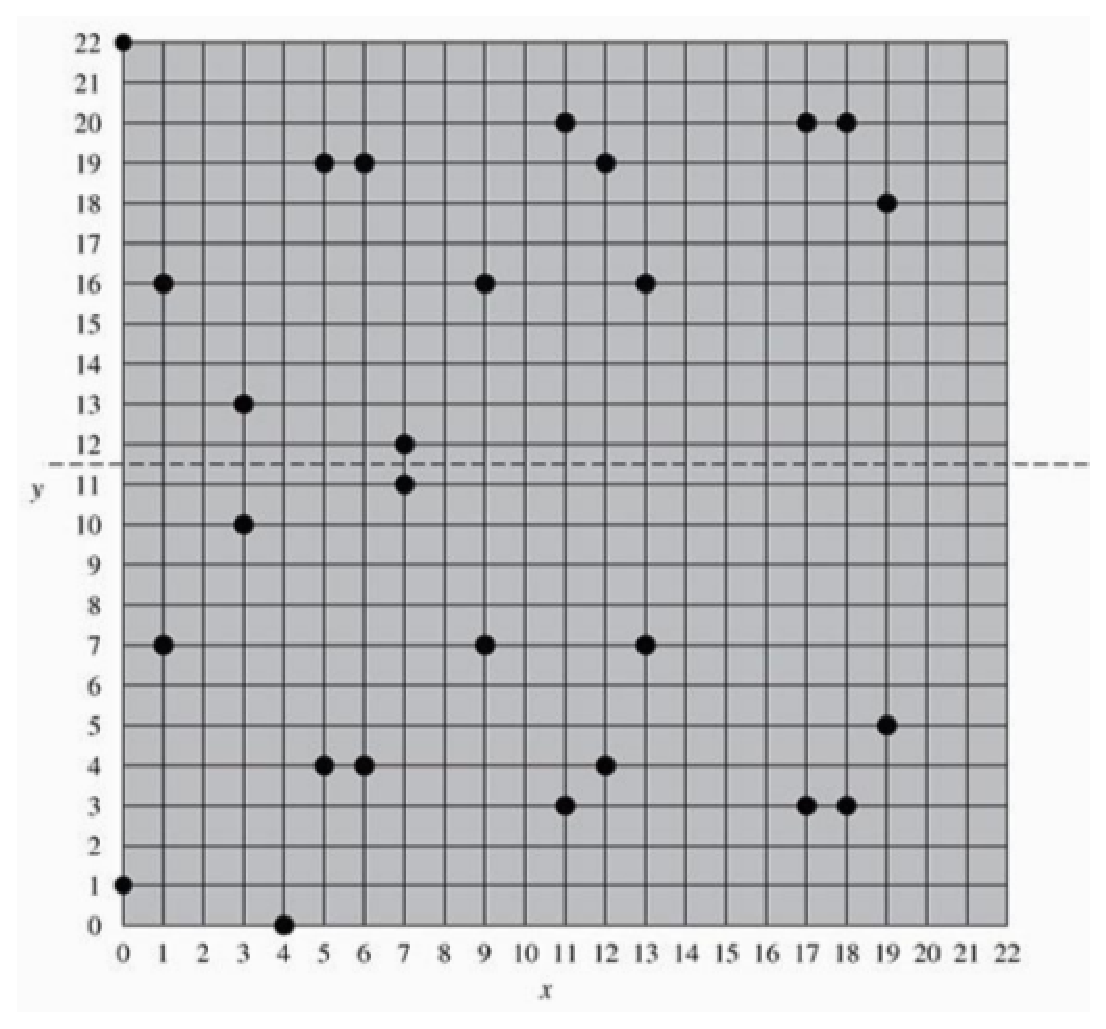
\includegraphics[scale=0.6, bb=0 0 515 478]{figuras/curva_sobre_corpo_finito.eps}
\caption{Curva elíptica $E_{23}(1, 1)$}
\label{fig:curva_exemplo}
\end{figure}

\begin{enumerate}
  \item $P + \mathcal{O} = P$.
  \item Se $P = (x_P, y_P)$, então $P + (x_P, -y_P) = \mathcal{O}$. O ponto $(x_P, -y_P)$ é o negativo de \(P\), indicado como \(-P\).
  \item Se $P = (x_P, y_P)$ e $Q = (x_Q, y_Q)$ com $P \neq -Q$, então $R = P + Q = (x_R, y_R)$ é determinado pelas seguintes regras:
    \begin{align}
    x_R &=(\lambda^2 - x_P - x_Q) \mod p \label{x_result} \\
    y_R &=(\lambda(x_P - x_R) - y_P) \mod p \label{y_result}
    \end{align}
  em que
    \begin{align}
    \label{lambda_result}
    \lambda =
    \begin{cases}
    \left(\dfrac{y_Q - y_P}{x_Q - x_P}\right) \mod p \textrm{, se} \ P \neq Q \\ \\
    \left(\dfrac{3x_P^2 + a}{2y_P}\right) \mod p \textrm{, se} \ P = Q
    \end{cases}
    \end{align}
  \item A multiplicação é definida como adição repetida; por exemplo, $4P = P + P + P + P$.
\end{enumerate}

Por exemplo, para somar os pontos $P(6, 19)$ e $(9, 16)$, pertencentes à curva $E_{23}(1, 1)$ descrita na Fig. (\ref{fig:curva_exemplo}), basta substituir os valores \(x_P = 6\), \(y_P = 19\), \(x_Q = 9\), \(y_Q = 16\), \(a = 1\) e \(p = 23\) nas Eqs. (\ref{x_result})
, (\ref{x_result}) e (\ref{lambda_result}) para obter como resultado da soma o ponto \(R = (9, 7)\). Para multiplicar o ponto $P(6,19)$ por 2, ou seja, ao somá-lo com ele mesmo, obtém-se como resultado \(2P = (13, 16)\).


% ORDEM DE UMA CURVA ELIPTICA
%
\subsection{Quantidade de pontos em uma curva elíptica}
Seja a curva elíptica $E$ definida sobre o corpo finito $\mathbb{F}_p$. O conjunto de todos os pontos que pertencem à curva elíptica é representado por $E(\mathbb{F}_p)$ (ver \ref{eq:pontosCurva}). A quantidade de pontos que compõe esse conjunto é a \textbf{ordem de $E$ sobre $\mathbb{F}_p$} e será representada pela notação $\#E(\mathbb{F}_p)$. \cite{Guide}

A ordem da curva elíptica é importante para o sistema criptográfico baseado em curvas elípticas, pois sua segurança depende dos fatores primos da ordem \cite{Alvarado:2005}. Se a ordem da curva elíptica pode ser fatorada em números primos pequenos, a sua segurança pode ser facilmente quebrada utilizando o algoritmo de Pohlig-Hellman, que não será abordado em profundidade nesse trabalho.

O teorema de Hasse fornece limites para a ordem de uma curva elíptica. Esse teorema determina que, sendo a curva elíptica $E$ definida sobre $\mathbb{F}_p$, então

\begin{equation}
p + 1 - 2\sqrt{p} \leq \#E(\mathbb{F}_p) \leq p + 1 + 2\sqrt{p}
\label{eq:HasseBounds}
\end{equation}

O \textbf{traço} de $E$ sobre $\mathbb{F}_p$ é $t = 2\sqrt{p}$. Sabendo-se o traço da curva definida sobre $\mathbb{F}_p$, é possível calcular a sua ordem. O algoritmo de Schoof (ver \ref{SchoofAlg}) calcula o traço de uma curva, permitindo saber a sua ordem.

%
% CRIPTOGRAFIA DE CURVAS ELÍPTICAS
%
\subsection{Criptografia de curvas elípticas} \label{sec:ecc}
Primeiro, selecione um inteiro grande \(p\) que seja primo e parâmetros da curva elíptica \(a\) e \(b\) de acordo com a Eq. (\ref{eq:5}) ou (\ref{eq:6}). Isso define o grupo de pontos $E_p(a, b)$. Em seguida escolha um ponto base $G \in E_p(a, b)$, cuja a ordem seja um valor muito grande \(n\). $E_p(a, b)$ e \(G\) são os parâmetros do criptossistema, conhecidos por todos os participantes.

Um acordo de chaves entre os usuários \textbf{A} e \textbf{B} pode ser realizado da seguinte maneira: \cite{Stallings:2011}
\begin{enumerate}
\item \textbf{A} seleciona um inteiro \(n_A < n\). Essa é chave privada de \textbf{A}, então \textbf{A} gera sua chave pública $P_A = n_A \times G$
\item Do mesmo modo, \textbf{B} seleciona um inteiro \(n_B < n\), sendo essa a chave privada de \textbf{B}. E então \textbf{B} calcula e divulga sua chave pública $P_B = n_B \times G$.
\item \textbf{A} e \textbf{B} agora podem compartilhar o mesmo ponto da curva elíptica, que será chamado de segredo compartilhado entre \textbf{A} e \textbf{B}. \textbf{A} obtém o segredo compartilhado através do cálculo $K = n_A \times P_B$. Da mesma forma, \textbf{B} obtém o segredo compartilhado através do cálculo $K = n_B \times P_A$
\end{enumerate}

É possível verificar que \textbf{A} e \textbf{B} chegam ao mesmo segredo compartilhado da seguinte forma
\begin{equation*}
n_A \times P_B = n_A \times (n_B \times G) = n_B \times (n_A \times G) = n_B \times P_A
\end{equation*}

Para quebrar esse esquema, um atacante precisa utilizar a curva $E_p(a, b)$ e o ponto base $G$, que são conhecidos, e uma das chaves públicas \(P_A\) ou \(P_B\) para descobrir respectivamente uma das chaves privadas \(n_A\) ou \(n_B\). Para isso, ele precisará encontrar um valor $x$ que satisfaça \(P_A = xG\), encontrando assim \(n_A = x\), ou \(P_B = xG\), encontrando \(n_B = x\). 

